\chapter{Example Generator Implementations}
To illustrate a few possibilities of BAG generators, we show various circuits of increasing complexity. 
\section{Starting Small: Passive Loaded Differential Amplifier}
A very commonly used block in many ICs is the differential amplifier. In the case the load is passive. The topology is the same as that used in Chapter 4, and can be seen in section 4.4. An example instance is shown in \ref{fig:passive_amp}.
\begin{figure}[h]
\centering
\begin{subfigure}{.8\linewidth}
  \centering
  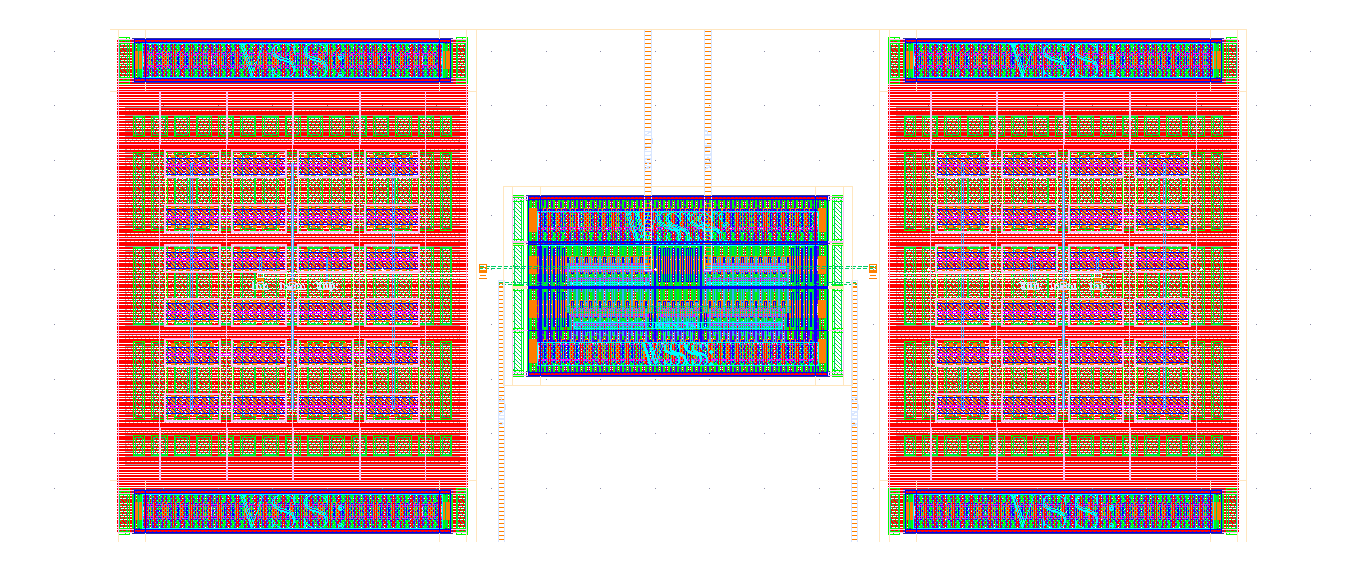
\includegraphics[width=\textwidth]{passive_layout}
  \caption{Full layout}
  \label{fig:sfig1}
\end{subfigure}
\begin{subfigure}{.8\linewidth}
  \centering
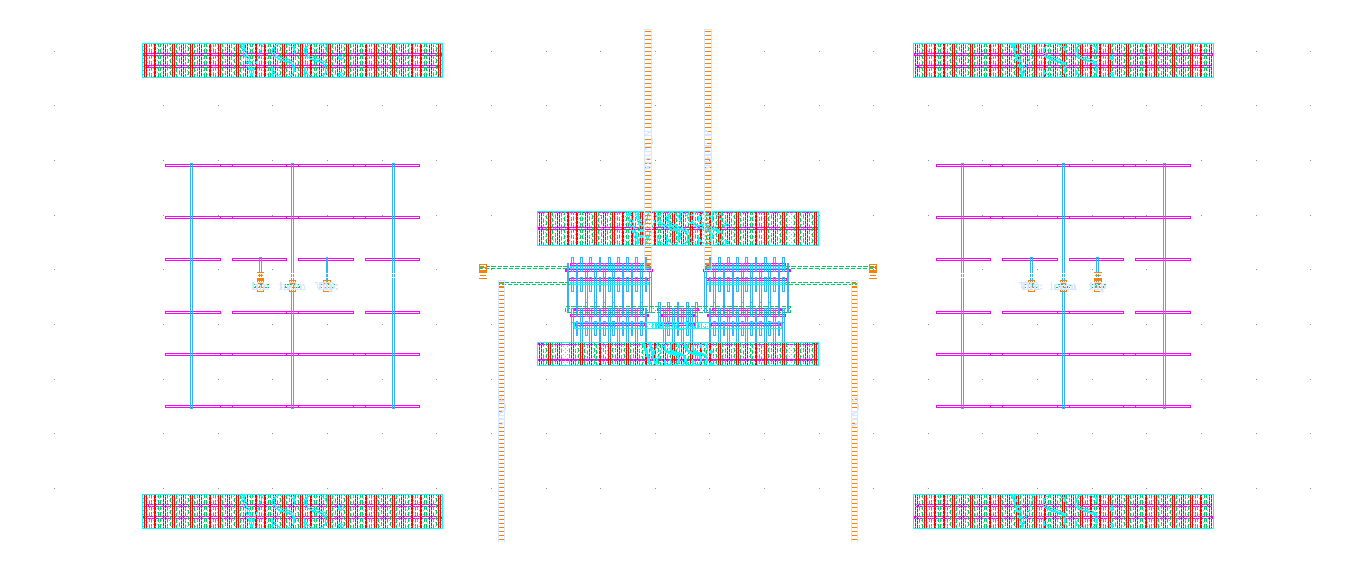
\includegraphics[width=\textwidth]{passive_layout_metals}
  \caption{Only the metals}
  \label{fig:sfig2}
\end{subfigure}
\caption{Differential amplifier layout}
\label{fig:passive_amp}
\end{figure}
\clearpage
All generators demonstrated have wire width parametrized so each type of wire (signal, bias, clock) can have a specific, customizable width. This generator additionally allows the user to specify resistor unit cell sizes, number of parallel and series units and transistor dimensions (width, fingers).

Another option is nearly identical, but with 3-bit resistor DACs instead of a single resistor as in \ref{fig:passive_dac}
\begin{figure}[h]
\centering
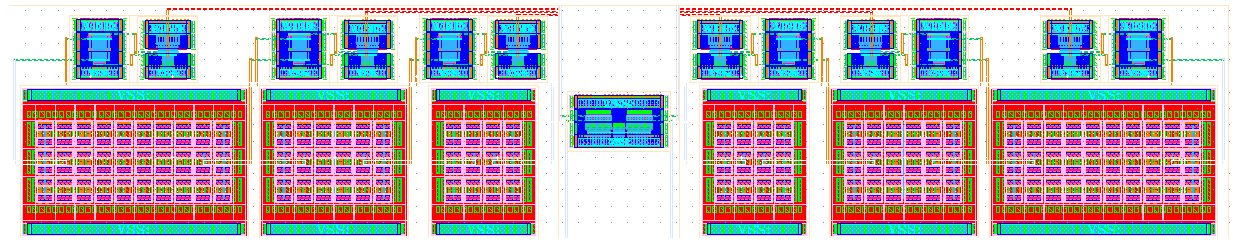
\includegraphics[width=\textwidth]{passive_dac}
\caption{Passive diff-amp with resistor DAC}
\label{fig:passive_dac}
\end{figure}

\section{Getting Fancier: A Double Tail Sense Amplifier and Latch}
Yet another crucial component in an analog receiver is the sampler. Before converting to purely digital processing, the received bits must be processed as either a 1 or a 0 through the use of a sampling circuit. While there are many ways to implement sampling, this report makes use of a double tail sense amp (DTSA). The schematic and operation are shown in Chapter 4. An example layout is shown in \ref{fig:dtsa_ex}.
\begin{figure}[h]
\centering
\begin{subfigure}{.4\linewidth}
  \centering
  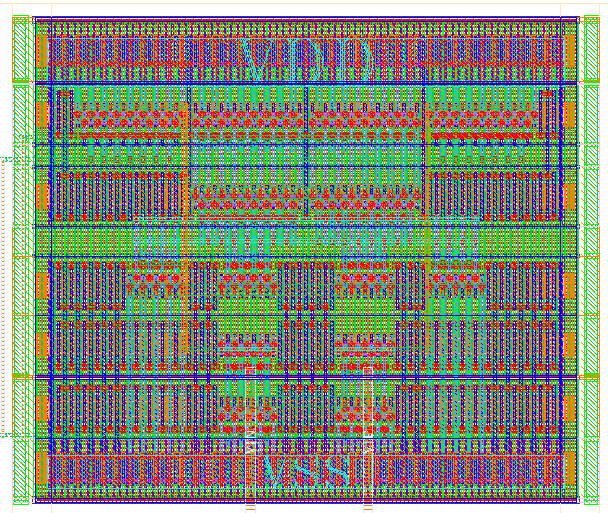
\includegraphics[width=0.8\textwidth]{dtsa_full}
  \caption{Full layout}
  \label{fig:sfig1}
\end{subfigure}
\begin{subfigure}{.4\linewidth}
  \centering
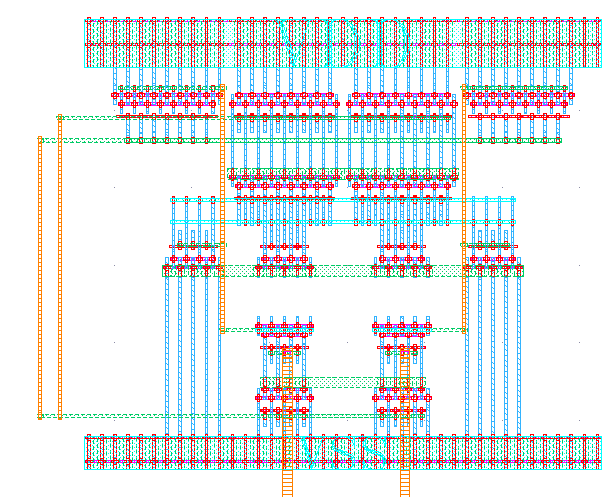
\includegraphics[width=0.8\textwidth]{dtsa_metal}
  \caption{Only the metals}
  \label{fig:sfig2}
\end{subfigure}
\caption{DTSA layout}
\label{fig:dtsa_ex}
\end{figure}
The DTSA block exemplifies even more of BAGs capability to include customization. In addition to all previously mentioned parametrization (wire widths, transistor sizings, etc.) this block also includes an option to generate input pair offset correction hardware. This hardware is implemented as a current that subtracts from the input pair's current during the integration step of operation (discussed more in  Chapter 4). The generator automatically accounts for how the setup changes when offset correction is included and automatically adds more pins/labels to the layout, as shown in \ref{fig:dtsa_enoc}.
\begin{figure}[h]
\centering
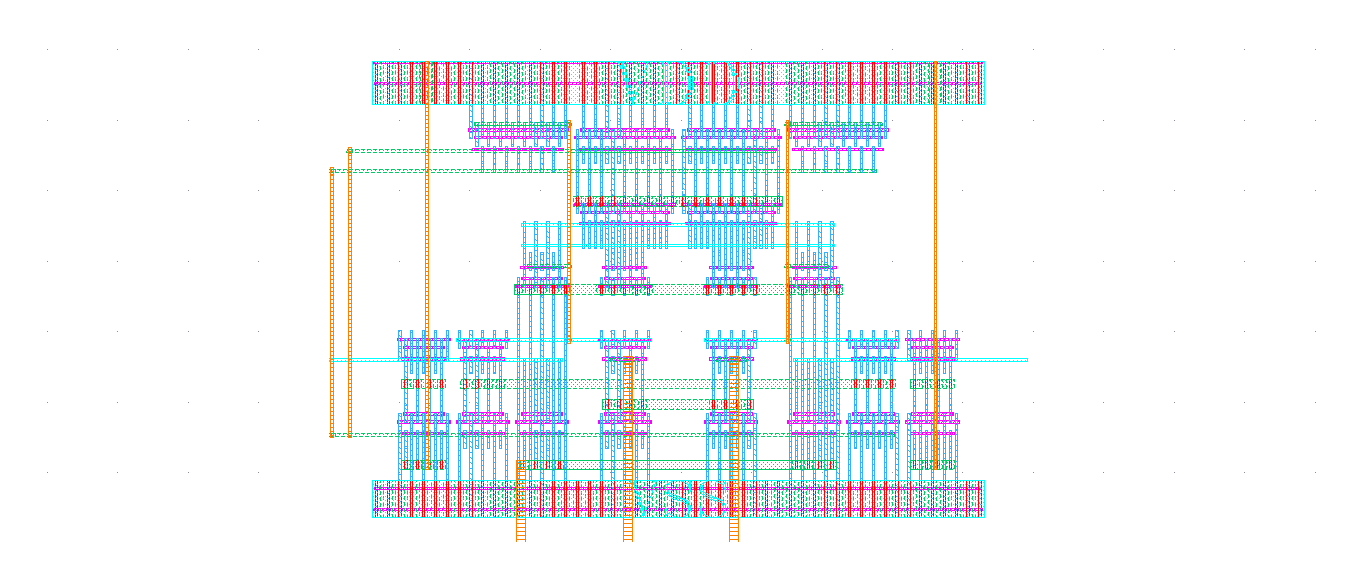
\includegraphics[width=\textwidth]{dtsa_metal_enoc}
\caption{DTSA with offset correction}
\label{fig:dtsa_enoc}
\end{figure}
Finally, the output of a comparator like this is only valid for a short time. We need a latch to store the value in between evaluation cycles. Thankfully, this is possible with BAG. Using TemplateBase we can attach a latch made previously to the output of the DTSA, like in \ref{fig:dtsa_d2s}.
\begin{figure}[h]
\centering
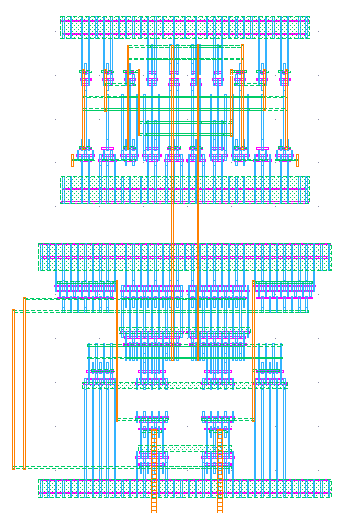
\includegraphics[width=0.4\textwidth]{dtsa_d2s}
\caption{DTSA with latch}
\label{fig:dtsa_d2s}
\end{figure}

\section{Endless Possibilities: An Entire Analog Front End Receiver or Two}
Manually creating the layout for an entire receiver (AFE) is a daunting process. As a final demonstration of how a user can start with small blocks and eventually create large, complex generators, two different front end architectures are shown. It is important to note that the size and complexity of these circuits makes is non-trivial, and would require significant manual work. These generators are capable of creating and extracting the entire layout in seconds, which truly allows faster design iteration by removing the bottleneck almost entirely. 

The first front end (\ref{fig:afe1}) is a chain of a TIA followed by a Cherry-Hooper amplifier stage, then a CTLE and two parallel preamplifiers. 
\begin{figure}[h]
\centering
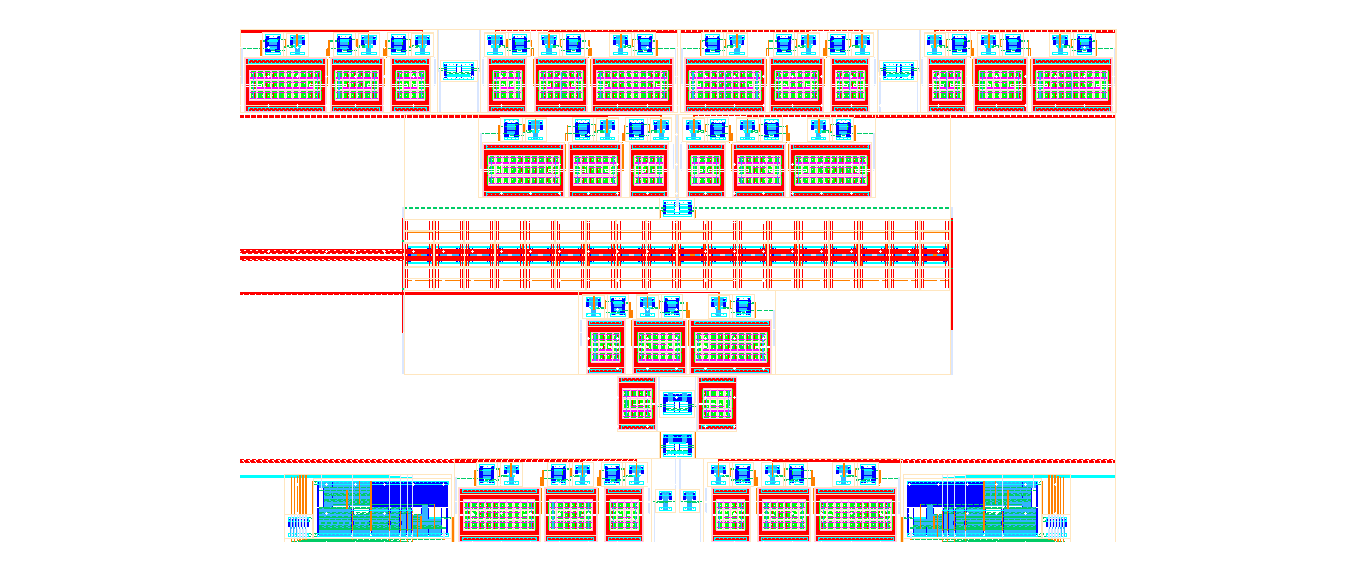
\includegraphics[width=0.3\textwidth]{afe1}
\caption{First front end}
\label{fig:afe1}
\end{figure}
There are also versions that include DACs for every passive element as well as current DACs for every bias input. There are versions that remove the Cherry-Hooper stage and include a comparator. 

Another example of a front end is the one that will be used in Chapter 4. This AFE is a quad data rate AFE similar to the previous AFE and is comprised of the chain: TIA, CTLE, 2x parallel passive diff amps, 4x samplers. The architecture and operation is explained in Chapter 4. The layout is shown in \ref{fig:afe2}.
\begin{figure}[h]
\centering
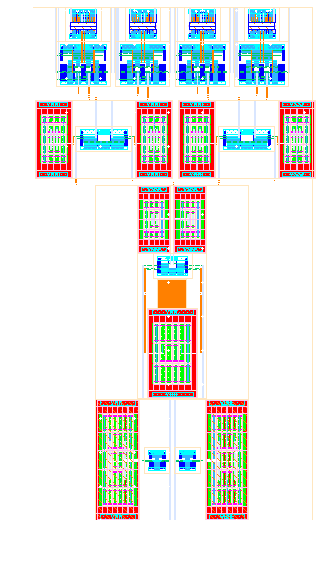
\includegraphics[width=0.3\textwidth]{afe2}
\caption{Second front end}
\label{fig:afe2}
\end{figure}
The main point of demonstrating these layouts is that with a library of ``leaf cells,'' composing large circuits is a very feasible task that would take an experienced user only one to two days to implement. With BAG, layout is no longer a painstaking process.

